We will now emperically validate that the hierarchical implementation is more time efficient than the standard implementation without sacrificying accuracy.
Two experiments will be conducted.

First, we will \textbf{measure elapsed time as insertions scale} of each implementation.
We anticpate that the hierarchical implementation will take less time than the standard implementation for any sufficiently large value of insertions.

Second, we will \textbf{measure false positives as we scale bits allocated per element} of each implementation.
We anticipate that the hierarchial and standard implementation will be approximately same as the theoerical false positive rate discussed before.

For each of these sections, we pseudorandomly generate keys to both insert and query.
Discussion on exactly how these keys are generated is discussed in the appendix.

%%%%%%%%%%%%%%%%%%%%%%%%%%%%%%%%%%%%%%%%%%
%%%%%%%%%%%%%%%%%%%%%%%%%%%%%%%%%%%%%%%%%%
%%%%%%%%%%%%%%%%%%%%%%%%%%%%%%%%%%%%%%%%%%

\subsection{Comparing Time Efficiency}

For this experiment, we seek to validate that the hierarchical implementation performs better than the standard implementation as the number of insertions grow.
\textit{Hypothesis:} The hierarchical bloom filter will take less time than the standard implementation to insert $n$ keys for any $n$.

\subsubsection{Experimental Settings}

The experiment will run as follows. For each implementaiton run the following procedure:
\begin{enumerate}
    \item Generate $n$ random keys.
    \item Generate a bloom filter of both varianets of size $10n$. Use the optimal theoeretical configuraiton for each bloom filter (i.e, $k=7$, $l=1$).
    \item Time how long it takes to insert all $n$ keys into each of the bloom filters. Report this number.
    \item Repeat for various sizes of $n$.
\end{enumerate}
Repeat this entire process $3$ times.

\subsubsection{Results}
\begin{center}
    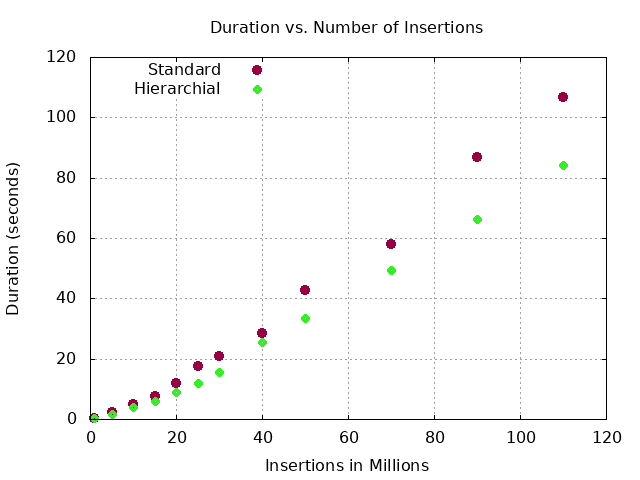
\includegraphics[width=13cm]{plots/scale-nm.png}
\end{center}
The slope of the line of best fits that are plotted are as follows whre $n$ is millions of insertions:
\begin{itemize}
    \item The best fit line for the standard implementation is: $t = 1.07146\cdot n - 5.83917$
    \item The best fit line for the hierarchical implementation is: $t = 0.789073\cdot n -3.64732 $
\end{itemize}
Thus, our experiment shows that the hierarchical implementation performs $35\%$ more operations per second than the standard implementation!

%%%%%%%%%%%%%%%%%%%%%%%%%%%%%%%%%%%%%%%%%%
%%%%%%%%%%%%%%%%%%%%%%%%%%%%%%%%%%%%%%%%%%
%%%%%%%%%%%%%%%%%%%%%%%%%%%%%%%%%%%%%%%%%%

\subsection{Comparing False Positive Rate}

For this experiment, we seek to validate that the hierarchical implementation does not have a worse false positive rate than the standard implementation.
\textit{Hypothesis:} We expect them to have approximately the same false positive rate as the theoeretical expectation discussed earlier.

\subsubsection{Experimental Settings}

The experiment will run as follows. 
\begin{enumerate}
\item Generate $150,000$ random ``insertion'' keys (of length 16).
\item Generate $150,000$ random ``false'' keys to query distinct from the insertion keys (of length 15).
\item For each implementaiton run the following procedure:
\begin{enumerate}
    \item Let $BPE$ be the bits per element (e.g $BPE = 1$ or $BPE = 10$).
    \item Generate a bloom filter of size $150,000\cdot BPE$.
    \item Insert all the `insertion'' keys and query all the ``false'' keys and measure how many of them the bloom filter return. Report this number.
    \item Repeat for various values of $BPE$.
\end{enumerate}
\item Repeat this procedure again $3$ times with different insertion and false keys.
\end{enumerate}

\subsubsection{Results}
\begin{center}
    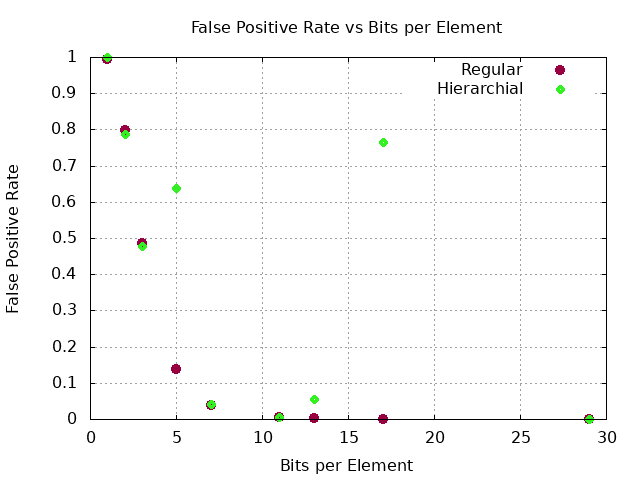
\includegraphics[width=14cm]{plots/fp.png}
\end{center}

As we can see, both the standard and hierarchical implementation closely match the theoeretical expectation. 
Both implementations do worse than theoeretically expected if bloom filters are overpacked, but after Bits per Elements is greater than 6, both implementations are very close to theoeretical expectation ($\pm -0.0005$) or better.

\subsection{Conclusion}
Our experiments have supported both of our theoretically justified hypothesises.
We have demonstrated that the hierarchical implementation is more efficient than the standard implementation; it can perform $35\%$ more operations per second!
Additionally, we have verified our that our implementation is just as effective as the standard implementation. 
